\documentclass[fleqn]{article}[11pt]
\usepackage{amsmath} 
\usepackage{nccmath} 
\usepackage{amssymb}
\usepackage[english]{babel}
\usepackage[autostyle]{csquotes}
\usepackage[margin=0.5in]{geometry}
\newcommand{\ds}{\displaystyle}
\usepackage{graphicx}
\usepackage{harpoon}
\usepackage[section]{placeins}

\begin{document}
	
\begin{center}\section*{MATH 316D W10}\end{center}
\subsection*{DD1 Individual Quiz}

\begin{enumerate}
	\item \textbf{Add}, ``Given the following 2$^{nd}$ order ODEs determine if they are linear or not. A linear operator by definition is of the form \(L(c_{1}u_{1}+c_{2}u_{2}+...+c_{n}u_{n})=c_{1}L[u_{1}]+c_{2}L[u_{2}]+...+c_{n}L[u_{n}]\)."
	
	\begin{enumerate}
		\item $r(t)\cfrac{d^2y(t)}{dt^2}+r'(t)\cfrac{dy(t)}{dt}+\lambda p(t)y(t)=1$ $\implies$ \textbf{Linear}
		\item $y\cdot y''-y=0$ $\implies$ \textbf{Linear}
		\item $(1-x^2)\cfrac{d^2y(x)}{dx^2}-2x\cfrac{dy(x)}{dx}+(\ \lambda-\cfrac{m^2}{(1-x^2)}\ )\ y(x)=0$ $\implies$ \textbf{Linear}
		\item $\cfrac{d^2y}{dt}+\cfrac{1}{\sin{y}}\cfrac{dy}{dt}-\ln{y}\ y=e^{-t}$ $\implies$ \textbf{Non-linear}
	\end{enumerate}
	
	\item \textbf{Keep} (previously question 1) but please make all the letters for the coefficients capitalized (i.e. A, B, C, and D).

	\item \textbf{Keep} (previously question 2).
	
	\item \textbf{Keep} (previously question 3).
	
	\item \textbf{Keep} (previously question 4) but the correct answer is not present. Please change the answers to:
		\begin{enumerate}
			\item $y_{h}(t)=c_1 e^{-2t}+c_2\, e^{-2t}$
			\item $y_{h}(t)=c_1 e^{-2t}+c_2\, te^{-2t}$ $\implies$ \textbf{Correct}
			\item $y_{h}(t)=c_1 e^{-4t}+c_2\, te^{-4t}$
			\item None of the above.
		\end{enumerate}
		
	\item \textbf{Keep} (previously question 5) and please make sure that all the answers have a subscripted `h'. Also please add an additional answer of "None of the above."
	
	\item \textbf{Keep} (previously question 6) but the correct answers are not present and the ODE is not typed correctly, please change the question and answers to:
	
	\(y''+2y'+3y=\sin{3t}\)
		\begin{enumerate}
			\item $y_{p}(t)=e^{-t}\ (c_1\ \cos{\sqrt{2}t}+c_2\ \sin{\sqrt{2}t})-\frac{1}{12}\ (\cos{3t}+\sin{3t})$
			\item $y_{p}(t)=-\frac{1}{6}\sin{3t}$
			\item $y_{p}(t)=-\frac{1}{12}\ (\cos{3t}+\sin{3t})$ $\implies$ \textbf{Correct}
			\item None of the above.
		\end{enumerate}
	
	\item \textbf{Keep} (previously question 7) but please add an additional answer of, ``None of the above."
	
	\item \textbf{Delete} (previously question 8).
\end{enumerate}

\subsection*{DD2 Group Quiz}

\begin{enumerate}
	\item \textbf{Change} to, ``Use the method of undetermined coefficients to find the particular solution to the following problems."
	
		\(y''+y'-2y=4t^2-1\)
			\begin{enumerate}
				\item $y_{p}(t)=c_{1}e^{-t}+c_{2}e^{2t}$
				\item $y_{p}(t)=-2t^2$
				\item $y_{p}(t)=-2t^2-2t-\frac{5}{2}$ $\implies$ \textbf{Correct}
				\item $y_{p}(t)=-2t^2+2t-\frac{5}{2}$
			\end{enumerate}
	
	\item \textbf{Change} to, 
	
		\(y''+4y'+3y=2t+4\cos{t}\)
			\begin{enumerate}
				\item $y_{p}(t)=\frac{2}{3}t+\frac{2}{5}\cos{t}+\frac{4}{5}\sin{t}$
				\item $y_{p}(t)=\frac{2}{3}t-\frac{8}{9}+\frac{2}{5}\cos{t}+\frac{4}{5}\sin{t}$ $\implies$ \textbf{Correct}
				\item $y_{p}(t)=c_{1}e^{-3t}+c_{2}e^{-t}$
				\item $y_{p}(t)=c_{1}e^{3t}+c_{2}e^{t}$
			\end{enumerate}
	
	\item \textbf{Change} to, ``Using the method of undetermined coefficients, find the general solution to the following problems."
	
		\(y''+3y'=3\sin{2t}\)
			\begin{enumerate}
				\item $y_{g}(t)=-\frac{9}{26}\cos{2t}-\frac{3}{13}\sin{2t}$
				\item $y_{g}(t)=c_{1}e^{-3t}+c_{2}-\frac{9}{26}\cos{2t}-\frac{3}{13}\sin{2t}$ $\implies$ \textbf{Correct}
				\item $y_{g}(t)=c_{1}e^{-3t}-\frac{9}{26}\cos{2t}-\frac{3}{13}\sin{2t}$
				\item None of the above.
			\end{enumerate}
	\item \textbf{Change} to,
	
		\(y''+4y'+3y=2t+4\cos{t}\)
			\begin{enumerate}
				\item $y_{g}(t)=\frac{2}{3}t-\frac{8}{9}+\frac{2}{5}\cos{t}+\frac{4}{5}\sin{t}$
				\item $y_{g}(t)=c_{1}e^{t}+c_{2}e^{3t}+\frac{2}{3}t-\frac{8}{9}+\frac{2}{5}\cos{t}+\frac{4}{5}\sin{t}$
				\item $y_{g}(t)=c_{1}e^{-t}+c_{2}e^{-3t}+\frac{2}{3}t-\frac{8}{9}+\frac{2}{5}\cos{t}+\frac{4}{5}\sin{t}$ $\implies$ \textbf{Correct}
				\item None of the above.
			\end{enumerate}

	\item \textbf{Change} to, ``Use the method of undetermined coefficients to find the solution to the following IVPs."
	
		\(y''+4y=2\sin{2t},\ y(0)=1,\ y'(0)=-1\)
			\begin{enumerate}
				\item $y(t)=\cos{2t}-\frac{1}{2}\sin{2t}$
				\item $y(t)=\cos{2t}-\frac{1}{2}\sin{2t}+4\cos{2t}-2\sin{2t}$
				\item $y(t)=\cos{2t}-\frac{1}{4}\sin{2t}-\frac{1}{2}t\cos{2t}$ $\implies$ \textbf{Correct}
				\item None of the above.
			\end{enumerate}

	\item \textbf{Change} to,
	
		\(y''+y'-y=3,\ y(0)=-1,\ y'(0)=-1\)
			\begin{enumerate}
				\item $y(t)=e^{\frac{t}{2}}\ (e^{\frac{\sqrt{5}t}{2}}+e^{\frac{-\sqrt{5}t}{2}})-3$
				\item $y(t)=e^{-\frac{t}{2}}\ (e^{\frac{\sqrt{5}t}{2}}+e^{\frac{-\sqrt{5}t}{2}})-3$ $\implies$ \textbf{Correct}
				\item $y(t)=e^{-\frac{t}{2}}\ (e^{\frac{\sqrt{5}t}{2}}+e^{\frac{-\sqrt{5}t}{2}})$
				\item None of the above.
			\end{enumerate}

\end{enumerate}

\subsection*{DD3 Weekly Quiz}

\begin{enumerate}
	\item \textbf{Change} to, ``For the following problems guess the form of the particular solution and choose the answer that most closely represents your guess."
	
		\(y''+4y=20e^{t}\cos{t}\)
			\begin{enumerate}
				\item $y_{p}(t)=e^{t}(Ae^{{i}t}+Be^{-{i}t})$
				\item $y_{p}(t)=Ae^{t}+B\cos{t}+C\sin{t}$
				\item $y_{p}(t)=Ae^{t}\cos{t}+Be^{t}\sin{t}$
				\item Both \textbf{\textup{a}} and \textbf{\textup{c}} satisfy the equation. $\implies$ \textbf{Correct}
				\item None of the above. 
			\end{enumerate}
	
	\item \textbf{Change} to,
	
		\(y'''+2y''-5y'+y=t^2+7\)
			\begin{enumerate}
				\item $y_{p}(t)=At^2$
				\item $y_{p}(t)=At^2+Bt+C$ $\implies$ \textbf{Correct}
				\item $y_{p}(t)=c_{1}e^{Root(r^{3}+2r^{2}-5r+1=0,1) t}+c_{2}e^{Root(r^{3}+2r^{2}-5r+1=0,2)t}+c_{3}e^{Root(r^{3}+2r^{2}-5r+1=0,3)t}$
				\item Both \textbf{\textup{a}} and \textbf{\textup{b}} satisfy the equation.
				\item None of the above. 
			\end{enumerate}
		
	\item \textbf{Change} to, ``For the following problems find the homogenous solution and simplify your answer (i.e. useing Euler's equation), then choose the answer that best represents your work."
	
		\(L\cdot q''(t)+R\cdot q'(t)+\cfrac{1}{C}\cdot q(t)=0\ ;\ L=10,\ R=40,\ C=\frac{1}{50}\)
			\begin{enumerate}
				\item $y_{h}(t)=c_{1}e^{(-2+i)t}+c_{2}e^{-(2+i)t)}$
				\item $y_{h}(t)=c_{1}e^{-t}+c_{2}e^{-3t}$
				\item $y_{h}(t)=e^{-2t}(c_{1}\cos{t}+c_{2}\sin{t})$ $\implies$ \textbf{Correct}
				\item None of the above.
			\end{enumerate}
			
	\item \textbf{Change} to,
	
		\(my''+\beta y'+ky=0;\ \beta^{2} < |k|;\ (\text{Hint: Let}\ \omega=\sqrt{4km-\beta^{2}}\ )\)
			\begin{enumerate}
				\item $y_{h}(t)=c_{1}e^{(\frac{-\beta+\sqrt{\beta^{2}-4km}}{2m})t}+c_{2}e^{{(\frac{-\beta-\sqrt{\beta^{2}-4km}}{2m}})t}$
				\item $y_{h}(t)=c_{1}e^{\frac{(-\beta+i\omega)t}{2m}}+c_{2}e^{\frac{-(\beta+i\omega)t}{2m}}$
				\item $y_{h}(t)=e^{-\frac{\beta t}{2m}}\ (c_{1}\cos{\frac{\omega t}{2m}}+c_{2}\sin{\frac{\omega t}{2m}})$ $\implies$ \textbf{Correct}
				\item None of the above.
			\end{enumerate}
		
	\item \textbf{Change} to, ``For the following problems find the particular solution using the method of undetermined coefficients and then choose the answer that best represents your work."
	
		\(y''+4y=20e^{t}\cos{t}\)
			\begin{enumerate}
				\item $y_{p}=5e^{t}\cos{t}$
				\item $y_{p}=e^{t}\ (4\cos{t}+2\sin{t})$ $\implies$ \textbf{Correct}
				\item $y_{p}=e^{t}\ (4\cos{t}-2\sin{t})$
				\item None of the above.
			\end{enumerate}
	
	\item \textbf{Change} to,
	
		\(y'''+2y''-5y'+y=t^{2}+7\)
			\begin{enumerate}
				\item $y_{p}=t^{2}$
				\item $y_{p}=t^{2}-10t+61$
				\item $y_{p}=t^{2}+10t+53$ $\implies$ \textbf{Correct} 
				\item None of the above.
			\end{enumerate}

	
	\item \textbf{Change} to, ``Solve the following IVPs using the method of undetermined coefficients and then choose the answer that best represents your work."
	
		\(y''+8y=\cos{2t};\ y(0)=1,\ y'(0)= \sqrt{2}\)
			\begin{enumerate}
				\item $y(t)=\frac{6}{7}\cos{2\sqrt{2}t}+\frac{1}{2}\sin{2\sqrt{2}t}+\frac{1}{7}\cos{t}$
				\item $y(t)=\frac{3}{4}\cos{2\sqrt{2}t}+\frac{1}{2}\sin{2\sqrt{2}t}+\frac{1}{4}\cos{2t}$ $\implies$ \textbf{Correct}
				\item $y(t)=-\frac{3}{4}\cos{2\sqrt{2}t}-\frac{1}{4}\sin{2\sqrt{2}t}+\frac{1}{4}\cos{2t}$
				\item None of the above.
			\end{enumerate}
	
	\item \textbf{Add}.
			
		\(y''-6y'+25y=50t^3-36t^2-63t+18;\ y(0)=1,\ y'(0)= 1\)
			\begin{enumerate}
				\item $y(t)=e^{3t}(\cos{4t} + \frac{1}{4}\sin{4t})+2t^{3}-3t$ $\implies$ \textbf{Correct}
				\item $y(t)=e^{3t}(\cos{4t} + \frac{1}{4}\sin{4t})+\frac{1}{2}t^{3}-t^{2}+\frac{54}{25}t+\frac{76}{625}$
				\item $y(t)=e^{7t} + \frac{1}{4}e^{-t}+2t^{3}-3t$
				\item None of the above.
			\end{enumerate}

		
	
	\item \textbf{Add} (essay question). 
	
		\begin{enumerate}
						\item ``Construct the general solution for the forced undamped spring-mass system by hand with $k=8$, $m=2$, and $F(t)=5\cos{2t}$. Determine the displacement of the mass at time $t$ if the system is set into motion with the initial conditions $y(0)=2$, $y'(0)=1$, then upload your work here." 

$\implies$ \textbf{Correct:} \boldmath{$y_{g}(t)=2\cos{2t}+\cfrac{1}{2}\sin{2t}+\cfrac{5}{8}\ t\sin{2t}$}
						\item ``Graph the solution to part \textbf{\textup{a}} using Mathematica and upload a picture of the graph here." 	\begin{figure}[h]
			\centering
				\graphicspath{{/Users/tylertrogden/Desktop/}}
				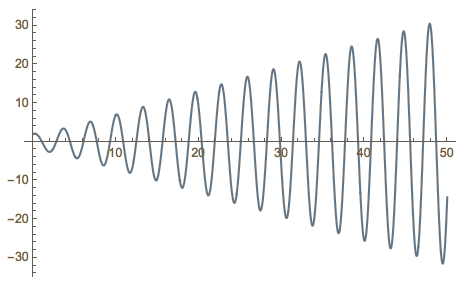
\includegraphics[height=2cm,width=4.5cm]{W10_WQ_Q9} $\implies$ \textbf{Correct}
		\end{figure} 

						\item ``Discuss the behavior of the spring-mass system as represented by the graph from part \textbf{\textup{b}}." An appropriate \textbf{answer} should be along the lines of, ``Since the system is undamped the max amplitude of the oscillations will grow unbounded forever, as seen in the graph of the solution, thus this is an unrealistic system."
						
		\end{enumerate}
	
	\item \textbf{Add} (essay question).
	
		\begin{enumerate}
			\item ``Construct the general solution by hand for an RLC circuit with external voltage source $E(t)=50\cos{40t}$, $L=10$, $R=40$, and $C=\cfrac{1}{50}$. Determine the current at time $t$ with the initial conditions $I(0)=100$, $I'(0)=25$,then upload your work here." 
			
			$\implies$ \textbf{Correct:} \boldmath{$y_{g}(t)=\cfrac{e^{-2t}}{20557}\ (2055444\cos{t}+4522733\sin{t})+\cfrac{1}{20557}\ (256\cos{40t}+2552\sin{40t})$}

			\item ``Graph the solution to part \textbf{\textup{a}} using Mathematica and upload a picture of the graph here." 	
				\begin{figure}[h]
					\centering
						\graphicspath{{/Users/tylertrogden/Desktop/}}				    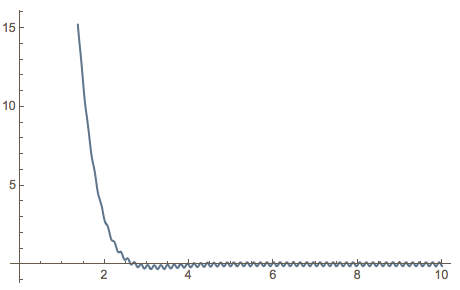
\includegraphics[height=3.75cm,width=4.5cm]{W10_WQ_Q10} $\implies$ \textbf{Correct}
				\end{figure} 

			\item ``Discuss the long-term behavior of the current as represented by the graph to part \textbf{\textup{b}}." An appropriate \textbf{answer} should be along the lines of, ``From the graph in part b, we can see that the RLC circuit is being powered by an alternating current which at time zero is very large but dies out quickly and is then governed by the forcing function (i.e. alternating current generator) at $t > 5$, approximately." 
			
		\end{enumerate}
\end{enumerate}

\end{document}